\documentclass[11pt]{article}
\usepackage[letterpaper,margin=0.85in]{geometry}
\setlength{\textfloatsep}{6pt plus 2pt minus 2pt}
\setlength{\intextsep}{6pt plus 2pt minus 2pt}
\setlength{\floatsep}{6pt plus 2pt minus 2pt}
\usepackage{times}

\usepackage{amsmath,amssymb,amsthm}
\usepackage{graphicx}
\usepackage{booktabs}
\usepackage{float}
\usepackage[table]{xcolor}
\usepackage{microtype}
\usepackage{hyperref}
\usepackage[capitalize,noabbrev]{cleveref}
\usepackage{enumitem}
\usepackage{algorithm}
\usepackage{algpseudocode}
\usepackage{tikz}
\usetikzlibrary{positioning,arrows.meta,calc}

% ---- CJE-safe macros (no geometry/spacing tweaks) ----
% Keep packages in main.tex; use this file only for \newcommand and theorem envs.

% --- Math helpers ---
\newcommand{\E}{\mathbb{E}}
\newcommand{\Var}{\operatorname{Var}}
\newcommand{\Cov}{\operatorname{Cov}}
\newcommand{\CV}{\operatorname{CV}}
\newcommand{\SE}{\operatorname{SE}}
\newcommand{\ESS}{\mathrm{ESS}}
\newcommand{\supp}{\operatorname{supp}}
\newcommand{\1}{\mathbf{1}}
\newcommand{\ind}[1]{\mathbf{1}_{#1}}

% argmin/argmax
\newcommand{\argmin}{\mathop{\mathrm{arg\,min}}\limits}
\newcommand{\argmax}{\mathop{\mathrm{arg\,max}}\limits}

% Norms & inner product (handy in proofs)
\newcommand{\norm}[1]{\left\lVert #1 \right\rVert}
\newcommand{\ip}[2]{\left\langle #1,\, #2 \right\rangle}

% --- Problem variables / notation ---
\newcommand{\X}{X}
\newcommand{\A}{A}
\newcommand{\Y}{Y}
\newcommand{\Sscore}{S}
\newcommand{\R}{\mathbb{R}}
\newcommand{\Rcal}{R}
\newcommand{\W}{W}

% Policies
\newcommand{\pzero}{\pi_0}
\newcommand{\pprime}{\pi'}

% Estimator tags (for small caps labels in text or tables)
\newcommand{\IPS}{\mathrm{IPS}}
\newcommand{\DR}{\mathrm{DR}}
\newcommand{\TMLE}{\mathrm{TMLE}}

% Optional: independence symbol
\newcommand{\indep}{\perp\!\!\!\perp}
\newcommand{\CI}{\mathrm{CI}}

% --- Theorem environments (requires amsthm in main.tex) ---
\newtheorem{theorem}{Theorem}
\newtheorem{lemma}{Lemma}
\newtheorem{prop}{Proposition}
\newtheorem{proposition}[prop]{Proposition} % shares counter with prop
\newtheorem{corollary}{Corollary}
\theoremstyle{remark}
\newtheorem{remark}{Remark}


\newcommand{\CJE}{\textsc{CJE}}
\newcommand{\RefuseLevel}{\textsc{Refuse-Level}}
\newcommand{\CVaR}{\mathrm{CVaR}}
\newcommand{\stoploss}[2]{\bigl(#1 - #2\bigr)_{+}}

\title{Lower-Tail Causal Judge Evaluation}
\author{}
\date{}

\begin{document}
\maketitle

\noindent\textbf{TLDR.} This appendix extends Causal Judge Evaluation so it can estimate how a policy behaves on its worst responses, not just on average. The motivation is simple. Two policies can have nearly the same average score and very different behaviour on the bottom slice that drives risk in deployment. The estimator reuses the same cheap judge and the same small batch of expensive oracle labels, and adds one extra piece that predicts how far the outcome falls short of a threshold. It comes with a check that refuses the estimate when the extra piece does not carry over from the labelled slice to the new policy. On real Arena data the check flags the adversarial policy and accepts the other three. Among the three it accepts, two policies that look identical on the average separate clearly on the deepest tail, which is the exact situation this extension is built to surface.

\section{Setup}

\CJE\ estimates a target policy's average outcome by training a cheap surrogate judge against a small slice of expensive oracle labels, and then averaging the judge's predictions over fresh responses from the target. The average is a fine summary for ranking, but it is the wrong summary for safety-relevant deployment, where two policies can have nearly the same average and very different lower tails. This appendix extends \CJE\ so that it can estimate that lower tail using the same data, the same calibrator, and the same audit gate.


Throughout, $\pzero$ and $\pprime$ are the logger and the target policy. Each row of data has a prompt $X$, a response $A$, a judge score $\Sscore$, and an oracle label $Y$. The lower-tail level $\alpha \in (0,1)$ controls how deep into the tail we are looking. We use $\alpha = 0.10$ throughout, meaning the worst tenth of responses. The $\alpha$-quantile of $Y$ under $\pprime$ is $q_\alpha(\pprime) = \inf\{t : \Pr_{\pprime}(Y \le t) \ge \alpha\}$, and the shortfall of $Y$ below a threshold $t$ is $\stoploss{t}{Y} = \max(t - Y, 0)$.

\section{Estimand}

The quantity we want is the average outcome under the target restricted to the worst $\alpha$-fraction of its responses:
\begin{equation}\label{eq:cvar-def}
\CVaR_\alpha(\pprime) \;=\; \E\!\big[Y(\pprime) \,\big|\, Y(\pprime) \le q_\alpha(\pprime)\big].
\end{equation}
At $\alpha = 1$ the formula recovers the policy mean. As $\alpha$ shrinks toward zero, the formula focuses on a deeper part of the tail. At $\alpha = 0.10$ it is the average outcome on the worst tenth of responses, the operating point we use throughout.\footnote{Conditional value at risk is the standard coherent risk measure in actuarial and risk-management practice. See Rockafellar and Uryasev, \emph{Optimization of conditional value-at-risk}, J.\ Risk 2(3), 2000.}

\begin{figure}[H]
\centering
\begin{minipage}{0.50\linewidth}\centering
\begin{tikzpicture}[
  node distance=0.30cm and 0.7cm, font=\scriptsize,
  every node/.style={align=center,inner sep=2.5pt},
  policy/.style={draw, rounded corners=2pt, minimum height=5.5mm, fill=white, font=\scriptsize},
  data/.style={draw, rounded corners=2pt, minimum height=5.5mm, fill=blue!8, font=\scriptsize},
  out/.style={draw, thick, rounded corners=2pt, minimum height=5.5mm, fill=orange!12, font=\scriptsize},
  >={Stealth[length=2.5pt]}
]
  \node[policy] (logger) {logger $\pzero$};
  \node[policy, below=of logger] (target) {target $\pprime$};
  \node[data, right=of logger] (oracle) {oracle slice $(\Sscore,Y)$};
  \node[data, right=of target] (fresh) {fresh draws ($\Sscore$)};
  \node[data, below=of fresh] (audit) {audit slice $(\Sscore,Y)$};
  \node[out, right=1.0cm of oracle] (cal) {\textbf{calibrator} $\hat g_t$};
  \node[out, right=1.0cm of cal] (est) {\textbf{CVaR} estimate};
  \node[out, right=1.0cm of audit] (aud) {\textbf{audit} $W_n$};
  \draw[->] (logger) -- (oracle);
  \draw[->] (target) -- (fresh);
  \draw[->] (target) -- (audit);
  \draw[->] (oracle) -- (cal);
  \draw[->] (cal) -- (est);
  \draw[->] (fresh) -| (est);
  \draw[->] (cal.south) -- (aud.north);
  \draw[->] (audit) -- (aud);
\end{tikzpicture}\par
\vspace{2pt}
\textit{(a) Data flow.}
\end{minipage}\hfill
\begin{minipage}{0.46\linewidth}\centering
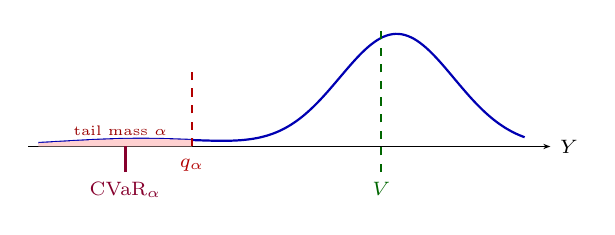
\begin{tikzpicture}[font=\scriptsize, >={Stealth[length=2.5pt]}, scale=0.65]
  \draw[->] (-0.2,0) -- (10,0) node[right] {$Y$};
  \draw[thick, blue!70!black, domain=0:9.5, samples=80, smooth]
        plot (\x, {2.2*exp(-0.4*(\x-7.0)*(\x-7.0)) + 0.15*exp(-0.2*(\x-2)*(\x-2))});
  \fill[red!18]
    plot[domain=0:3.0, samples=40, smooth]
        (\x, {2.2*exp(-0.4*(\x-7.0)*(\x-7.0)) + 0.15*exp(-0.2*(\x-2)*(\x-2))})
    -- (3.0,0) -- (0,0) -- cycle;
  \draw[red!70!black, thick, dashed] (3.0,0) -- (3.0,1.6);
  \node[red!70!black, below] at (3.0,-0.05) {$q_\alpha$};
  \node[red!60!black, font=\tiny] at (1.6,0.30) {tail mass $\alpha$};
  \draw[purple!70!black, thick] (1.7,-0.5) -- (1.7,0);
  \node[purple!70!black, below] at (1.7,-0.5) {$\CVaR_\alpha$};
  \draw[green!40!black, thick, dashed] (6.7,-0.5) -- (6.7,2.3);
  \node[green!40!black, below] at (6.7,-0.5) {$V$};
\end{tikzpicture}\par
\vspace{2pt}
\textit{(b) CVaR vs.\ mean.}
\end{minipage}
\end{figure}

\section{Estimator}

We cannot use \cref{eq:cvar-def} as a recipe for an estimate, because the threshold $q_\alpha(\pprime)$ is unknown and we observe relatively few outcomes from the target. We need to rewrite the same quantity in a form we can compute from the data we do have. There is a standard identity that does this. The same lower-tail value can be written as the maximum of a one-parameter expression over a candidate threshold $t$,
\begin{equation}\label{eq:cvar-dual}
\CVaR_\alpha(\pprime) \;=\; \sup_{t \in \R} \Big\{\, t \;-\; \tfrac{1}{\alpha}\, \E_{\pprime}\!\big[\stoploss{t}{Y}\big] \,\Big\},
\end{equation}
and the maximiser is exactly $q_\alpha(\pprime)$. This is useful because the expression inside the maximisation is a mean of a deterministic function of $Y$, which is the kind of object \CJE's existing Direct estimator was built to handle.

The estimator has three pieces. For each candidate threshold $t$ on a grid, we fit a calibrator on the oracle slice that takes a judge score and predicts the conditional expected shortfall of $Y$ below $t$. We apply that calibrator to the judge scores of fresh responses under $\pprime$ and take the empirical mean, which estimates the inner expectation in \cref{eq:cvar-dual}. We then maximise over the grid. \cref{alg:cvar} states the procedure together with the audit, after both have been described.

\section{Audit}

A CVaR estimate from \cref{alg:cvar} can be wrong for two distinct reasons. The first is that $\hat t$, the threshold the algorithm picks, may not actually be the $\alpha$-quantile of $Y$ under $\pprime$. The second is that the calibrator $\hat g_{\hat t}$, which we fit on the oracle slice, may behave differently on the target policy than it did on the oracle slice, in the sense that its prediction of the conditional expected shortfall is wrong on average for $\pprime$. The audit checks each cause with one moment, evaluated on a held-out audit slice that has both the judge score and the oracle label observed.

The first audit moment is
\begin{equation}\label{eq:g1}
g_1(O; \hat t, \alpha) \;=\; \1\{Y \le \hat t\} - \alpha.
\end{equation}
This is the gap between the share of audit observations that fall at or below the chosen threshold and the nominal level $\alpha$. If $\hat t$ is the $\alpha$-quantile of $Y$ under $\pprime$, then by definition exactly an $\alpha$-fraction of audit observations should fall at or below it, and $g_1$ averages to zero in expectation. A non-zero average of $g_1$ on the audit slice is direct evidence that $\hat t$ is not the right threshold.

The second audit moment is
\begin{equation}\label{eq:g2}
g_2(O; \hat t) \;=\; \stoploss{\hat t}{Y} \;-\; \hat g_{\hat t}(\Sscore).
\end{equation}
This is the residual between the actual shortfall of $Y$ below $\hat t$ on the audit slice and the calibrator's prediction of that shortfall. If the calibrator works under the target as well as it works on the oracle slice, the prediction equals the conditional expected shortfall under $\pprime$, and the residual averages to zero in expectation. A non-zero average residual on the audit slice is direct evidence that the calibrator does not transfer.

We combine the two moments into one test. Let $\bar g$ be the average of $(g_1, g_2)$ over the audit slice and let $\hat\Sigma$ be an estimate of its covariance matrix. We describe the variance estimator in the next section. The two moments are typically correlated because the same observations contribute to both, so we use the full covariance rather than the diagonal and the test reweights them by their joint variability. The Wald statistic is the quadratic form
\begin{equation}\label{eq:wald}
W_n \;=\; \bar g^{\top} \hat\Sigma^{-1} \bar g.
\end{equation}
When both moments are zero in expectation,\footnote{This is the threshold-indexed analogue of the main paper's mean-transport condition $\textbf{(T1)}$. It reduces to that condition in the limit $\alpha \to 1$.} $W_n$ behaves in large samples like a chi-squared random variable with two degrees of freedom, and a value above the $5\%$-level critical value is evidence that one of the two conditions has failed. We treat such a rejection as a signal to recalibrate or to refuse making a level claim about $\CVaR_\alpha(\pprime)$, mirroring how the main paper uses its own audit gate for the policy mean.

\section{Inference}

The confidence interval for the CVaR estimate uses the cluster bootstrap with $B = 500$ replicates. In each replicate we resample prompt clusters in the calibration slice and the fresh-draw set, refit the calibrator $\hat g_t$ for every threshold on the grid, recompute the estimator, and report the central $95\%$ of the resulting bootstrap distribution. Refitting the calibrator inside each replicate is what makes the interval honest in this setting: when the oracle slice is small, the calibrator itself is the dominant source of uncertainty, and an interval that pretended otherwise would be too narrow. We use the bootstrap rather than an analytical formula because the estimator is the maximum of an objective that is not smooth in $t$, and writing a closed-form variance would require quantities (the density of $Y$ at the quantile, derivatives of the calibrator) that are harder to estimate than the variance itself.

The variance estimator $\hat\Sigma$ for the audit's Wald statistic uses the same paired bootstrap, with one essential addition. The threshold $\hat t_b$ is also re-found inside each replicate, by re-running the maximisation, rather than being held at its original value. The reason is the same non-smoothness: if we held $\hat t$ fixed in the bootstrap, the resulting variance estimate would miss the contribution of $\hat t$ to the variability of $\bar g$, and the test would be miscalibrated.\footnote{The variance under a re-estimated nuisance is the framework of Chen, Linton, and Van Keilegom (2003), \emph{Estimation of semiparametric models when the criterion function is not smooth}, Econometrica 71(5), Theorem~B.}

\begin{algorithm}[H]
\caption{Direct CVaR-CJE estimator and transport audit.}
\label{alg:cvar}
\begin{algorithmic}[1]
\Statex \textbf{Estimator.} Inputs: oracle slice $\{(\Sscore_j, Y_j)\}_{j=1}^{m}$; fresh-draw judge scores $\{\Sscore_i\}_{i=1}^{n}$ under $\pprime$; level $\alpha$; grid $\mathcal{G}$ of $61$ candidate thresholds anchored at the oracle-side $\alpha$-quantile of $Y$.
\For{$t \in \mathcal{G}$}
  \State $\hat g_t \gets$ non-increasing isotonic regression\footnotemark{} of $\stoploss{t}{Y_j}$ on $\Sscore_j$
  \State $\bar Z_t \gets \tfrac{1}{n} \sum_{i=1}^{n} \hat g_t(\Sscore_i)$
\EndFor
\State $\hat t \gets \arg\max_{t \in \mathcal{G}} \big(\, t - \bar Z_t/\alpha \,\big)$
\State \Return $\widehat\CVaR_\alpha^{\,\mathrm{Direct}}(\pprime) = \hat t - \bar Z_{\hat t}/\alpha$
\Statex
\Statex \textbf{Audit.} Additional input: audit slice $\{(\Sscore_k, Y_k)\}_{k=1}^{n_a}$ under $\pprime$.
\State $g_{1,k} \gets \1\{Y_k \le \hat t\} - \alpha$
\State $g_{2,k} \gets \stoploss{\hat t}{Y_k} - \hat g_{\hat t}(\Sscore_k)$
\State $\bar g \gets$ mean of $(g_{1,k}, g_{2,k})$ across $k$
\State $\hat\Sigma \gets$ paired bootstrap covariance of $\bar g$ over $B$ replicates, refitting $\hat g_t$ and re-running the maximisation for $\hat t_b$ inside each replicate
\State \Return $W_n = \bar g^{\top} \hat\Sigma^{-1} \bar g$; reject if $W_n > \chi^2_{2,\,0.95}$
\end{algorithmic}
\end{algorithm}
\footnotetext{We use scikit-learn's pool-adjacent-violators implementation, \texttt{IsotonicRegression(increasing=False)}. The non-increasing shape constraint reflects that a higher judge score should predict a smaller shortfall.}

\section{Arena results}
\label{sec:results}

We re-run the main paper's Arena experiment with no change to the data, the oracle slice, the fold structure, the calibrator, or the fresh-draw mechanism. The only addition is the new CVaR column, which applies \cref{alg:cvar} on top of the same calibrator that produces the Mean column. The Mean column reproduces the paper's headline \emph{direct$+$cov} estimator. We aggregate twenty oracle-slice seeds at $n = 5{,}000$ fresh draws per policy, with $25\%$ oracle coverage and $5$-fold cross-fitting. The table below reports per-target estimates at $\alpha = 0.10$ with median per-seed $95\%$ CIs in brackets. The Audit $p$ and Reject rate columns refer to the CVaR Wald audit of \cref{eq:wald}, not the main paper's mean audit.

\begin{table}[H]
\centering
\setlength{\tabcolsep}{4pt}
\resizebox{\linewidth}{!}{%
\begin{tabular}{lrrrrrr}
\toprule
Target $\pprime$ &
$\widehat V_{\mathrm{Direct}}(\pprime)$ &
$V(\pprime)$ truth &
$\widehat\CVaR_{0.10}^{\,\mathrm{Direct}}(\pprime)$ &
$\CVaR_{0.10}(\pprime)$ truth &
Audit $p$ &
Reject rate \\
\midrule
% AUTOFILL-START
\texttt{parallel}                                & 0.772 [0.764, 0.780] & 0.771 & 0.255 [0.230, 0.283] & 0.267 & $0.60$       & $5\%$  \\
\texttt{premium}                                 & 0.765 [0.758, 0.773] & 0.762 & 0.251 [0.228, 0.278] & 0.257 & $0.35$       & $0\%$  \\
\texttt{clone}                                   & 0.761 [0.754, 0.769] & 0.762 & 0.249 [0.223, 0.276] & 0.269 & $0.59$       & $5\%$  \\
\texttt{unhelpful}                               & 0.421 [0.299, 0.514] & 0.143 & 0.036 [0.019, 0.098] & 0.000 & ${<}10^{-8}$ & $95\%$ \\
% AUTOFILL-END
\bottomrule
\end{tabular}
}
\end{table}

The CVaR estimates separate the policies cleanly. The three benign policies all score around $0.25$ on the worst tenth of responses, roughly a third of their mean. The unhelpful policy scores essentially zero on the same tail. That is the difference the mean column does not show: not a quantitative gap, but a categorical one. The worst tenth of unhelpful responses is uniformly bad, while the worst tenth of the others is mediocre but non-zero.

Pooling all rows of the run, the absolute error against the ground truth is larger when the audit rejects than when it accepts, and the audit's $p$-value is negatively correlated with the absolute error. The audit filters which estimates to trust.

The mean and the lower-tail summary disagree on some pairs. The table below sweeps the tail level across $\alpha \in \{0.20, 0.10, 0.05, 0.01\}$. The \texttt{clone} and \texttt{premium} policies share essentially the same mean of $0.762$, yet at $\alpha = 0.01$ their CVaR truths are $0.072$ and $0.090$, a gap the mean cannot see.

\begin{table}[H]
\centering
\setlength{\tabcolsep}{5pt}
\begin{tabular}{lrcccc}
\toprule
Policy & $V$ truth & $\widehat\CVaR_{0.20}\,/\,\text{truth}$ & $\widehat\CVaR_{0.10}\,/\,\text{truth}$ & $\widehat\CVaR_{0.05}\,/\,\text{truth}$ & $\widehat\CVaR_{0.01}\,/\,\text{truth}$ \\
\midrule
\texttt{clone}     & 0.762 & $0.369\,/\,0.376$ & $0.249\,/\,0.269$ & $0.171\,/\,0.169$ & $0.075\,/\,0.072$ \\
\texttt{premium}   & 0.762 & $0.373\,/\,0.397$ & $0.251\,/\,0.257$ & $0.173\,/\,0.180$ & $0.075\,/\,0.090$ \\
\texttt{parallel}  & 0.771 & $0.379\,/\,0.406$ & $0.255\,/\,0.267$ & $0.173\,/\,0.175$ & $0.074\,/\,0.079$ \\
\texttt{unhelpful} & 0.143 & $0.061\,/\,0.000$ & $0.036\,/\,0.000$ & $0.025\,/\,0.000$ & $0.018\,/\,0.000$ \\
\bottomrule
\end{tabular}
\end{table}

\appendix
\section{Monte Carlo evidence}
\label{app:mc}

To check that the audit and the bootstrap interval behave correctly under known truth, we build a synthetic data-generating process from the Arena data. For each policy we use the empirical $Y$ marginal, fit a monotone curve relating $\Sscore$ to the conditional mean of $Y$, and add Gaussian noise with $Y$-quartile-dependent variance. For the adversarial \texttt{unhelpful} policy we add a mixture component placing about a third of the probability mass at $Y = 0$. A scalar dial $\delta$ shifts the target's lower-tail conditional mean downward, so $\delta = 0$ is the well-specified null.

\subsection{The Wald audit's null distribution}
\label{app:wald-mc}

The first check asks whether the audit's test statistic actually follows the chi-squared distribution with two degrees of freedom we claimed in \cref{eq:wald}. We sample calibration and audit slices from the same DGP at base$\to$base, $\delta = 0$, with three hundred outer replicates and eighty inner bootstrap reps per audit. The procedure is below. The table reports moments and quantiles of the empirical $W_n$ distribution against the chi-squared target at two audit sample sizes. The KS row is the Kolmogorov--Smirnov distance between the empirical CDF of $W_n$ and the chi-squared CDF, with the corresponding $p$-value on the row below.

\begin{algorithm}[H]
\caption{Wald audit calibration MC at base$\to$base, $\delta = 0$.}
\label{alg:wald-mc}
\begin{algorithmic}[1]
\Statex Inputs: base DGP. calibration size $m$. audit size $n_a$. replicates $R$.
\For{$r = 1, \dots, R$}
  \State Draw calibration $\{(\Sscore_j, Y_j)\}_{j=1}^{m}$ from base DGP
  \State Draw audit $\{(\Sscore_k, Y_k)\}_{k=1}^{n_a}$ from base DGP
  \State Run \cref{alg:cvar} to obtain $\hat t_r$ and Wald statistic $W_r$
\EndFor
\State Compare empirical CDF of $\{W_r\}$ to $\chi^2_2$ via KS, moments, and quantiles
\end{algorithmic}
\end{algorithm}

The message is that the audit's null distribution is correctly calibrated, and so the $5\%$ refusal gate fires at the rate the user expects when transport actually holds. This works because the bootstrap variance captures the contribution of the threshold $\hat t$ to the variability of $\bar g$. A sample covariance on the audit slice alone, which holds $\hat t$ fixed, would miss that piece and the test would be too aggressive.

\begin{table}[H]
\centering
\setlength{\tabcolsep}{8pt}
\begin{tabular}{lrrr}
\toprule
Statistic & $n_a = 1{,}000$ & $n_a = 2{,}500$ & target ($\chi^2_2$) \\
\midrule
Mean                                  & $1.79$  & $1.97$  & $2.000$ \\
Median                                & $1.385$ & $1.30$  & $1.386$ \\
Variance                              & $2.97$  & $3.94$  & $4.000$ \\
$95$th percentile                     & $5.21$  & $5.30$  & $5.991$ \\
KS statistic                          & $0.070$ & $0.054$ & \\
KS $p$-value                          & $0.098$ & $0.325$ & \\
Reject rate at $\alpha = 0.05$         & $0.037$ & $0.030$ & $0.050$ \\
\bottomrule
\end{tabular}
\end{table}

\subsection{Each moment catches its own failure}
\label{app:moment-isolation}

The audit has two moments because there are two ways the estimate can be wrong, and we would like each to fail in isolation. We use two controlled perturbations on top of the well-specified DGP, with $200$ replicates per cell at $n_a = 2{,}000$. In \emph{Mode A} we evaluate the audit at $\hat t + \Delta$ instead of $\hat t$. The calibrator at the shifted threshold is still well-specified, so $g_2$ has zero mean by construction and only $g_1$ moves. In \emph{Mode B} we add a constant $c$ to every calibrator prediction inside the audit. The dual's argmax is invariant to a constant shift, so $\hat t$ is unchanged and $g_1$ stays at its baseline while only $g_2$ moves. In the table below, the mean-$g_1$ and mean-$g_2$ columns confirm that each perturbation hits only the intended moment.

\begin{table}[H]
\centering
\setlength{\tabcolsep}{8pt}
\begin{tabular}{lrrr}
\toprule
Cell & mean $g_1$ & mean $g_2$ & reject rate \\
\midrule
baseline (both hold)                & $+0.002$ & $+0.000$ & $0.08$ \\
Mode A: $\Delta = +0.02$             & $+0.013$ & $+0.000$ & $0.22$ \\
Mode A: $\Delta = +0.05$             & $+0.029$ & $+0.000$ & $0.68$ \\
Mode B: $c = +0.005$                 & $+0.002$ & $-0.005$ & $0.87$ \\
Mode B: $c = +0.010$                 & $+0.002$ & $-0.010$ & $1.00$ \\
\bottomrule
\end{tabular}
\end{table}

The mean-$g_1$ and mean-$g_2$ columns confirm that each perturbation hits only the intended moment, and the reject rate climbs in both directions. Either failure on its own is enough to fire the audit, which is what gives the test its power against the realistic case where a wrong calibrator drags the threshold off with it.

\subsection{Audit reject rate and confidence-interval coverage}
\label{app:semi-synth-mc}

A wider sweep confirms the picture across the four target policies. We run $2{,}500$ outer replicates over $25$ cells at $\alpha = 0.10$ and $n = 2{,}000$, with $100$ replicates per cell, varying target policy and $\delta$. The procedure is below.

\begin{algorithm}[H]
\caption{Semi-synthetic MC at target $\pprime$, level $\alpha$, dial $\delta$.}
\label{alg:semi-mc}
\begin{algorithmic}[1]
\Statex Inputs: per-policy DGPs. replicates $R$. sample sizes $m, n, n_a$.
\State $C^\star \gets $ population $\CVaR_\alpha(\pprime)$ under the DGP
\For{$r = 1, \dots, R$}
  \State Draw calibration $\{(\Sscore_j, Y_j)\}_{j=1}^{m}$ from base DGP
  \State Draw fresh-draw $\{\Sscore_i\}_{i=1}^{n}$ and audit $\{(\Sscore_k, Y_k)\}_{k=1}^{n_a}$ from $\pprime$'s DGP at mis-spec $\delta$
  \State Run \cref{alg:cvar} to obtain $\widehat\CVaR_r$, cluster-bootstrap CI $[\ell_r, u_r]$, and audit decision $A_r$
  \State Record $A_r$ and the coverage indicator $\1\{\ell_r \le C^\star \le u_r\}$
\EndFor
\State Aggregate to per-cell reject rate, unconditional coverage, and audit-gated coverage
\end{algorithmic}
\end{algorithm}

The left block of the table below reports the audit reject rate at the $5\%$ level as $\delta$ rises. The right block reports the bootstrap interval's coverage of the true $\CVaR_{0.10}$ at $\delta = 0$, both unconditionally and conditional on the audit accepting. For reference, the cleanest base$\to$base null at $\delta = 0$ has unconditional CI coverage $0.93$ and audit-gated coverage $0.95$, with the audit accepting on $94$ of $100$ replicates. The bootstrap interval is honest only on the subset where the audit accepts, and on that subset the empirical coverage hits the nominal rate.

\begin{table}[H]
\centering
\setlength{\tabcolsep}{4.5pt}
\begin{tabular}{lrrrrr|rrr}
\toprule
$\pprime$ & $\delta=0$ & $\delta=0.02$ & $\delta=0.05$ & $\delta=0.10$ & $\delta=0.20$ & all reps & $\mid$accept & accept \\
\midrule
\texttt{clone}                      & $0.06$ & $0.04$ & $0.09$ & $0.22$ & $0.70$ & $0.78$ & $0.81$ & $94/100$ \\
\texttt{premium}                    & $0.07$ & $0.08$ & $0.11$ & $0.19$ & $0.70$ & $0.92$ & $0.94$ & $93/100$ \\
\texttt{parallel}                   & $0.10$ & $0.15$ & $0.21$ & $0.36$ & $0.78$ & $0.89$ & $0.89$ & $90/100$ \\
\texttt{unhelpful}                  & $0.90$ & $0.89$ & $0.75$ & $0.83$ & $0.78$ & $0.18$ & $1.00$ & $10/100$ \\
\bottomrule
\end{tabular}
\end{table}


\end{document}
